\documentclass{beamer}

% --- Core fonts & language (no CJK) ---
\usepackage[T1]{fontenc}
\usepackage[english]{babel}
\usepackage{lmodern}

% --- Math, algorithms, graphics, colors, tikz ---
\usepackage{amsmath,amssymb}
\usepackage{algorithm}
\usepackage{algorithmic}
\usepackage{graphicx}
\usepackage{subcaption}
\usepackage{caption}
\usepackage{tikz}
\usetikzlibrary{overlay-beamer-styles}
\usepackage{booktabs,multicol,stackengine}
\usepackage[table,dvipsnames]{xcolor} % dvipsnames enables ForestGreen
\usepackage{cancel}
\usepackage{moresize}

% --- Hyperref ---
\usepackage{hyperref}

% --- Listings (code) ---
\usepackage{listings}
\definecolor{nus-orange}{RGB}{239,124,0}
\definecolor{nus-blue}{RGB}{0,61,124}
\definecolor{halfgray}{gray}{0.55}

\lstset{
  basicstyle=\ttfamily\footnotesize, % use \scriptsize if you need more lines on a slide
  keywordstyle=\bfseries\color{nus-blue},
  stringstyle=\color{ForestGreen},
  numbers=left,
  numberstyle=\scriptsize\color{halfgray},
  rulesepcolor=\color{nus-orange},
  frame=shadowbox,
  columns=flexible,
  showstringspaces=false,
  keepspaces=true,
  tabsize=2,
  breaklines=true
}

% --- English labels (to match BT5110_tutorial9) ---
\renewcommand{\figurename}{Figure}
\renewcommand{\algorithmname}{Algorithm}

% --- Your style & macros (keep in same folder) ---
\usepackage{SHU}
% VITAL STUFF
\renewcommand\epsilon\varepsilon
\renewcommand\phi\varphi
\renewcommand\leq\leqslant
\renewcommand\geq\geqslant
\newcommand\defeq{\stackrel{\mathrm{def}}{=}}

% For revision
\newcommand\rev[1]{{#1}}

% COMMENTS
\newcommand\mikael[1]{\textcolor{orange}{[\textbf{Mikaël:} #1]}}
\newcommand\pierre[1]{\textcolor{magenta}{[\textbf{Pierre:} #1]}}
\newcommand\pratik[1]{\textcolor{blue}{[\textbf{Pratik:} #1]}}

% SMOL SYMBOLS
\newcommand\calF{\mathcal{F}}
\newcommand\RR{\mathbb{R}}
\newcommand\QQ{\mathbb{Q}}
\newcommand\bD{\mathbf{D}}

% REDUCTIONS
\newcommand{\tr}{\leq_{\mathsf{P}}}
\newcommand{\equivt}{\equiv_{\mathsf{P}}}

% PROBLEMS
\newcommand\escore{\mathsf{EScore}}
\newcommand\score{\mathsf{Score}}
\newcommand\eshapley{\escore_{\cshapley}}
\newcommand\shapley{\score_{\cshapley}}
\newcommand\ebanzhaf{\escore_{\cbanzhaf}}
\newcommand\banzhaf{\score_{\cbanzhaf}}
\newcommand\ev{\mathsf{EV}}
\newcommand\evs{\mathsf{EV}_\star}
\newcommand\ennv{\mathsf{ENV}} % \env was already defined
\newcommand\envss{\mathsf{ENV}_{\star,\star}}
\newcommand\mc{\mathsf{MC}}
\newcommand\env{\mathsf{ENV}}

% NOTATIONS
\newcommand\vars{\mathsf{Vars}}
\newcommand\out{\mathsf{out}} % for output gate
\newcommand\cshapley{c_{\mathrm{Shapley}}}
\newcommand\cbanzhaf{c_{\mathrm{Banzhaf}}}
\newcommand\ar{\mathsf{ar}}
\newcommand\const{\mathsf{Const}}
\newcommand{\pqe}{\mathrm{PQE}}
\newcommand\prov{\mathrm{Prov}}

% For algorithm2e
\newcommand{\hrulealg}[0]{\vspace{1mm} \hrule \vspace{1mm}}

% For alignment of numbers
\newcommand{\0}{\phantom{0}}

% Example
\newcommand{\phiex}{\phi_{\mathrm{ex}}}


% --- Title block (BT5110 look) ---
\title{BT5110: Tutorial 1 — Entity- - Relationship Model}
\author{\href{https://pratik2358.github.io/}{Pratik Karmakar}}
\institute{School of Computing,\\ National University of Singapore}
\date{AY25/26 S1}

\begin{document}
\begin{frame}
  \titlepage
  \IfFileExists{nus-logo.png}{
    \begin{figure}[htpb]\centering
      
\includegraphics[keepaspectratio, scale=0.18]{nus-logo.png}
    \end{figure}
  }{}
\end{frame}

\begin{frame}
    \begin{figure}
        \centering
        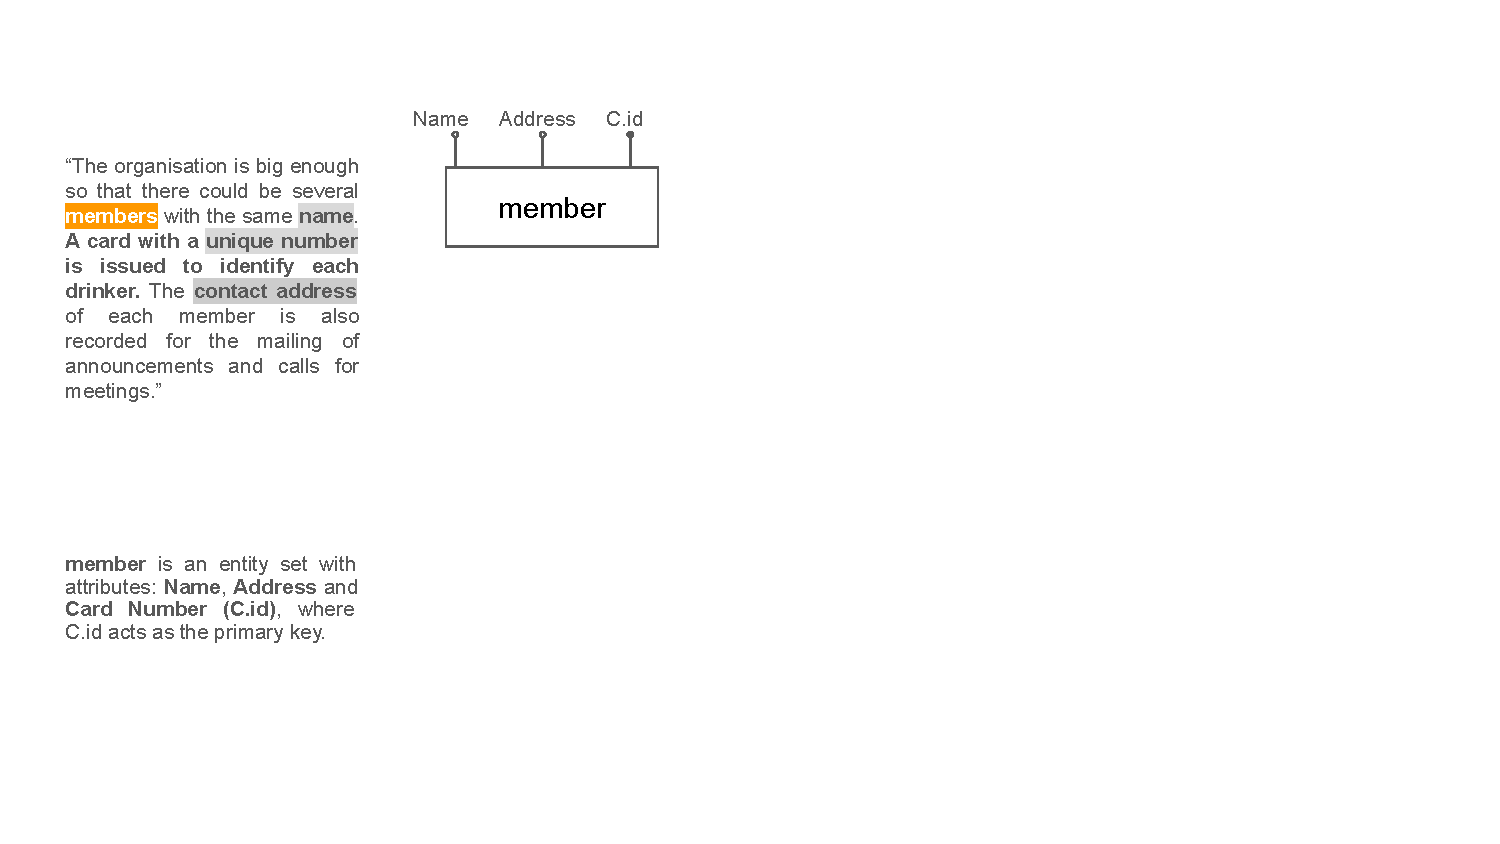
\includegraphics[width=1.1\linewidth]{tut_02_files/01.pdf}
    \end{figure}
\end{frame}

\begin{frame}
    \begin{figure}
        \centering
        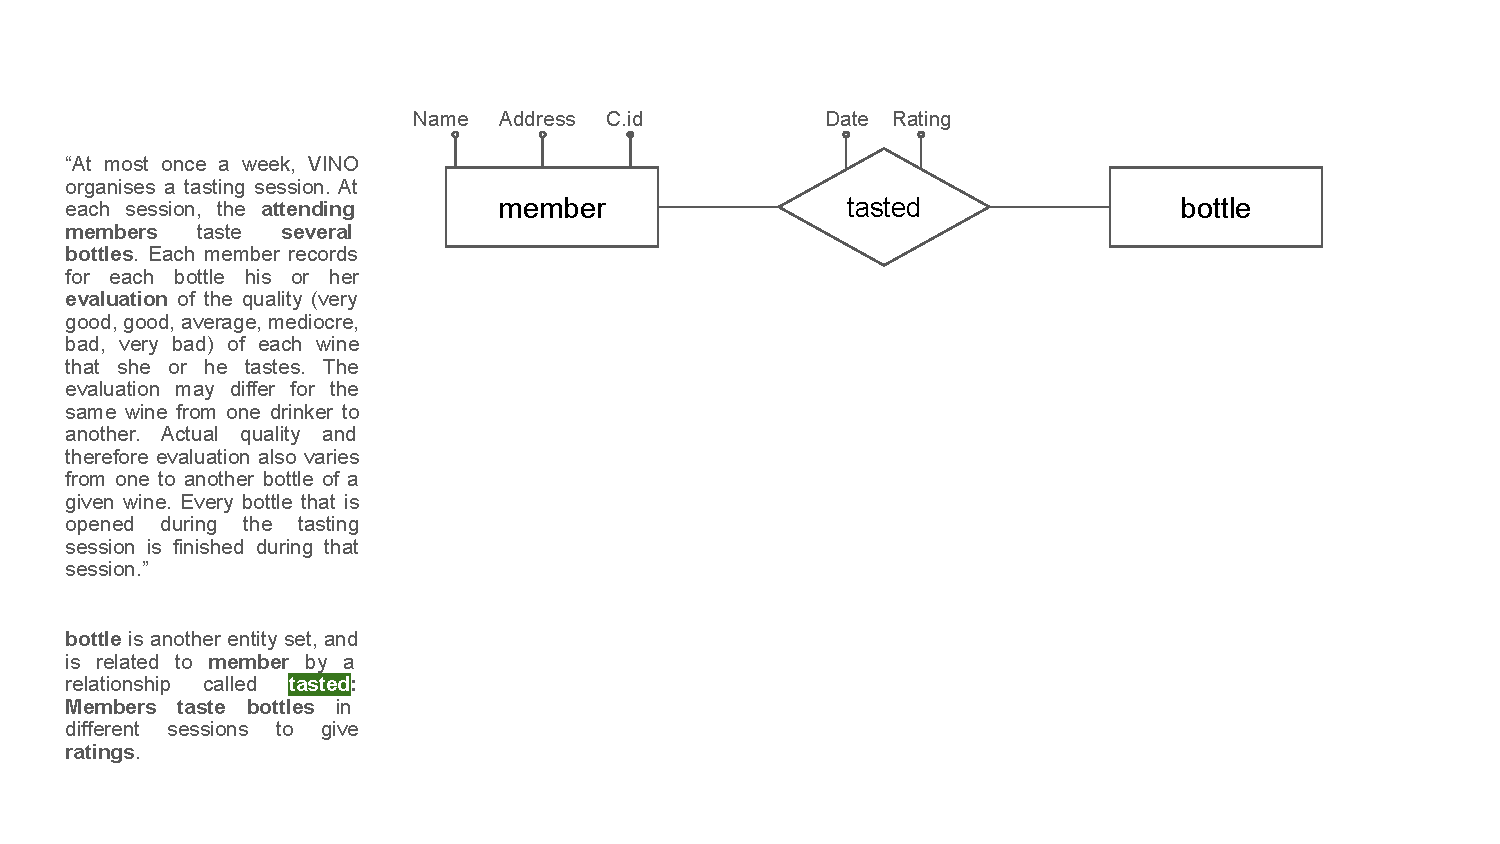
\includegraphics[width=1.1\linewidth]{tut_02_files/02.pdf}
    \end{figure}
\end{frame}

\begin{frame}
    \begin{figure}
        \centering
        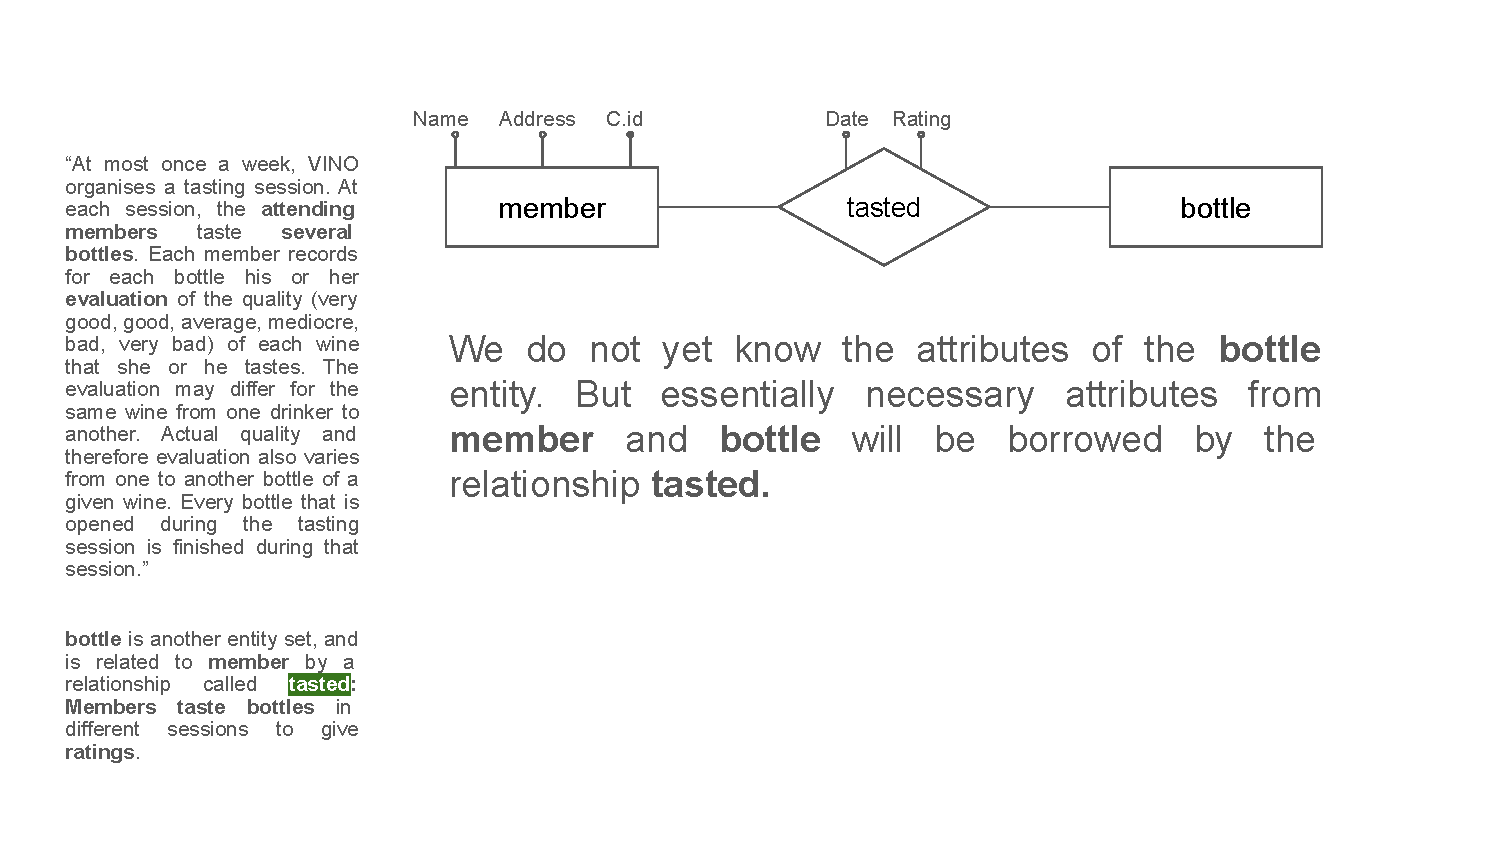
\includegraphics[width=1.1\linewidth]{tut_02_files/03.pdf}
    \end{figure}
\end{frame}

\begin{frame}
    \begin{figure}
        \centering
        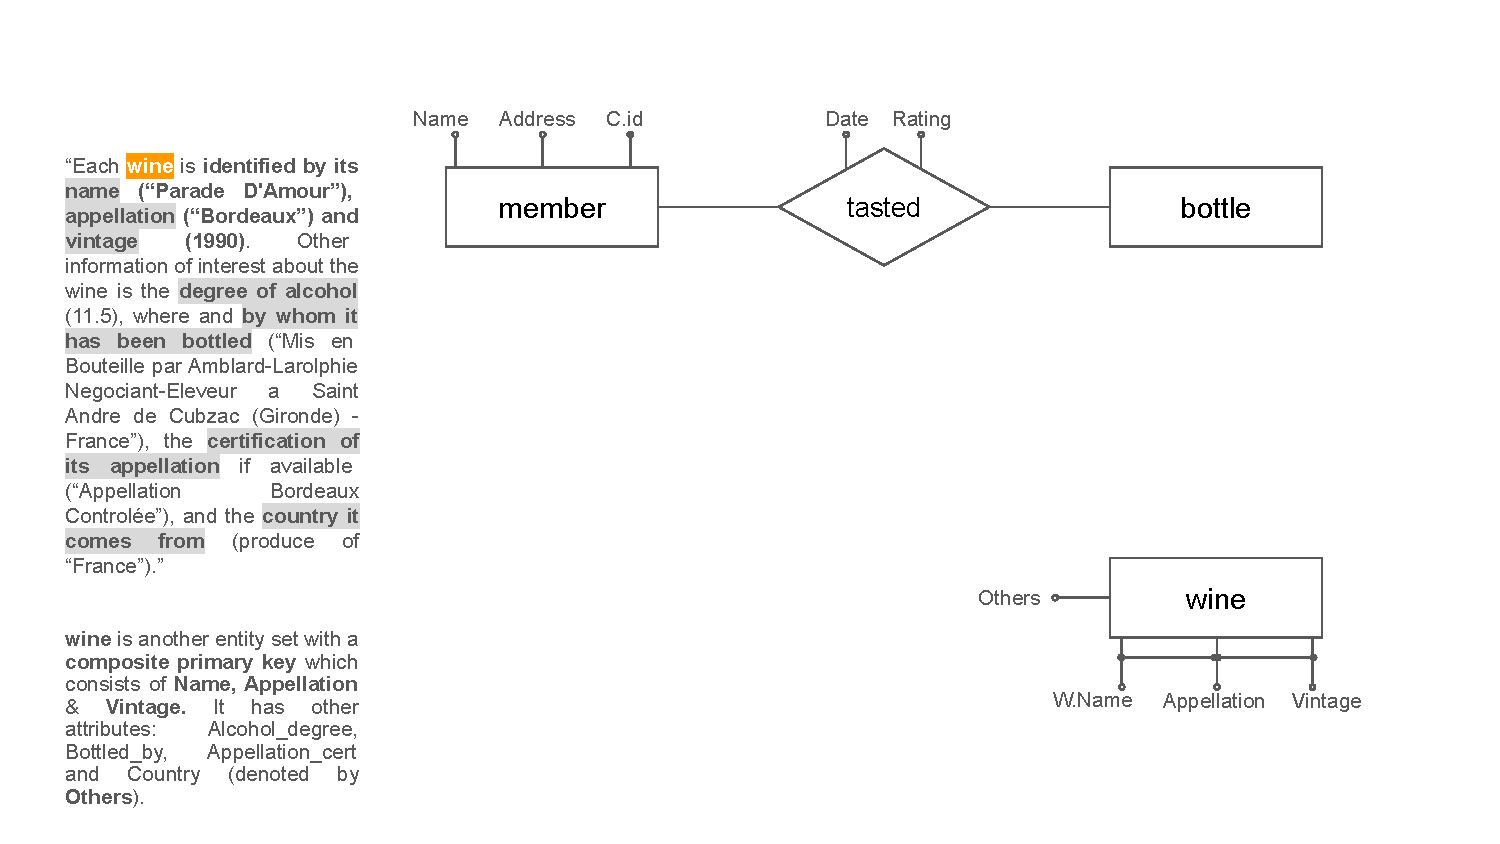
\includegraphics[width=1.1\linewidth]{tut_02_files/04.pdf}
    \end{figure}
\end{frame}

\begin{frame}
    \begin{figure}
        \centering
        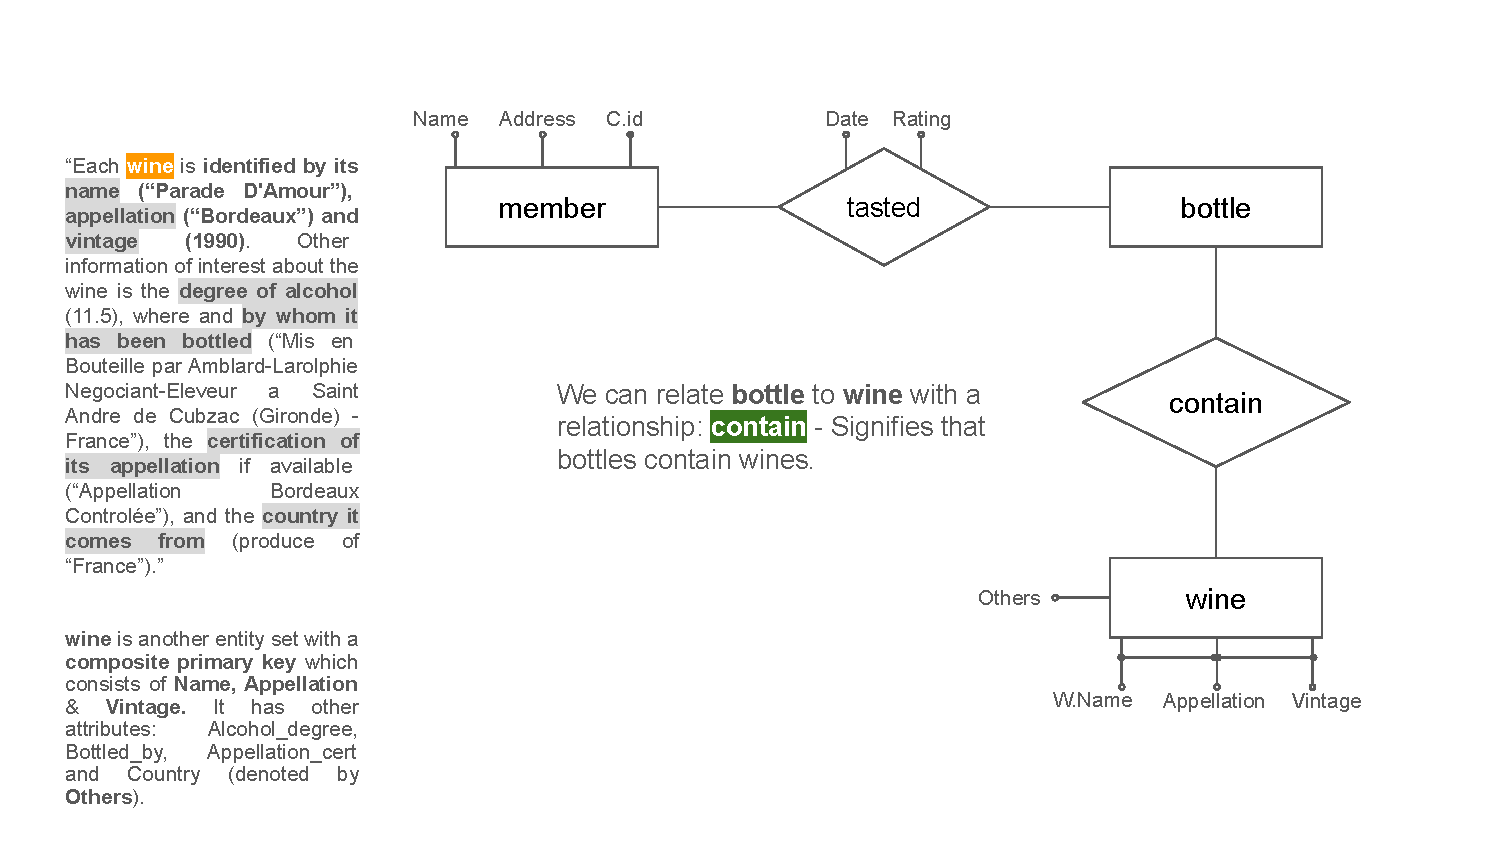
\includegraphics[width=1.1\linewidth]{tut_02_files/05.pdf}
    \end{figure}
\end{frame}

\begin{frame}
    \begin{figure}
        \centering
        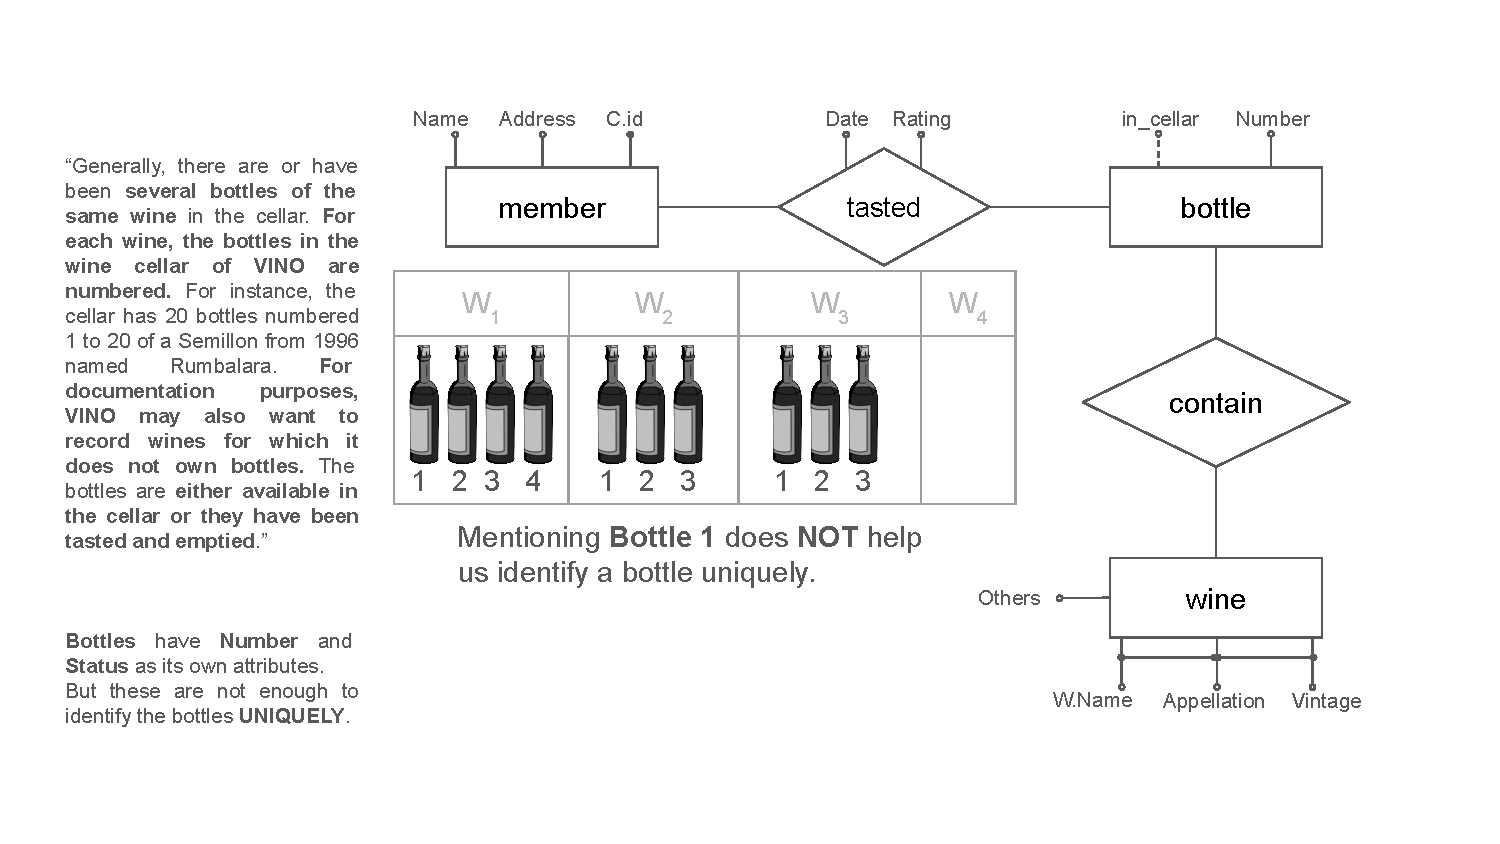
\includegraphics[width=1.1\linewidth]{tut_02_files/06.pdf}
    \end{figure}
\end{frame}

\begin{frame}
    \begin{figure}
        \centering
        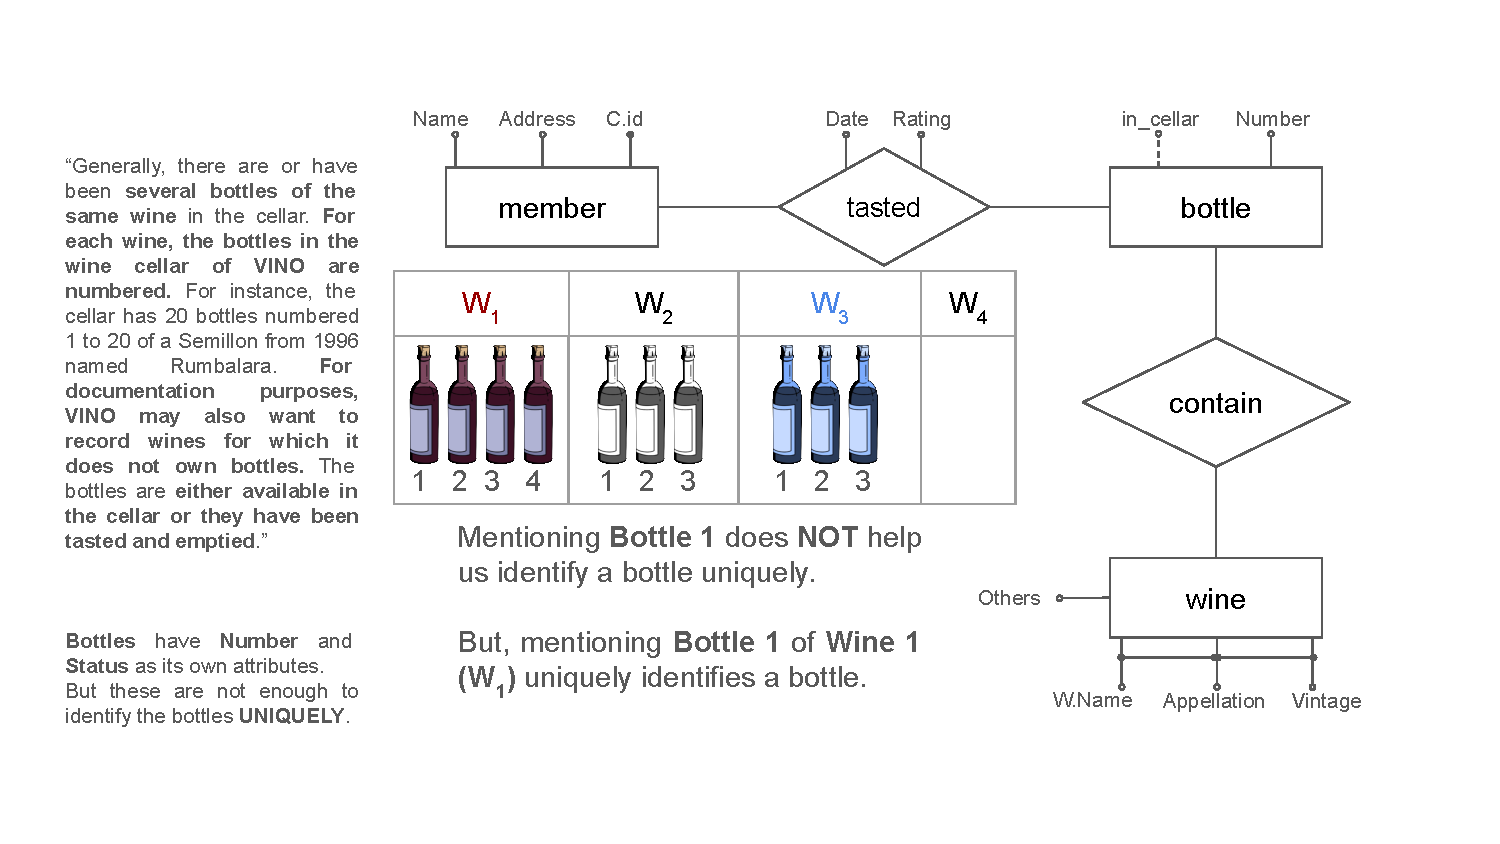
\includegraphics[width=1.1\linewidth]{tut_02_files/07.pdf}
    \end{figure}
\end{frame}

\begin{frame}
    \begin{figure}
        \centering
        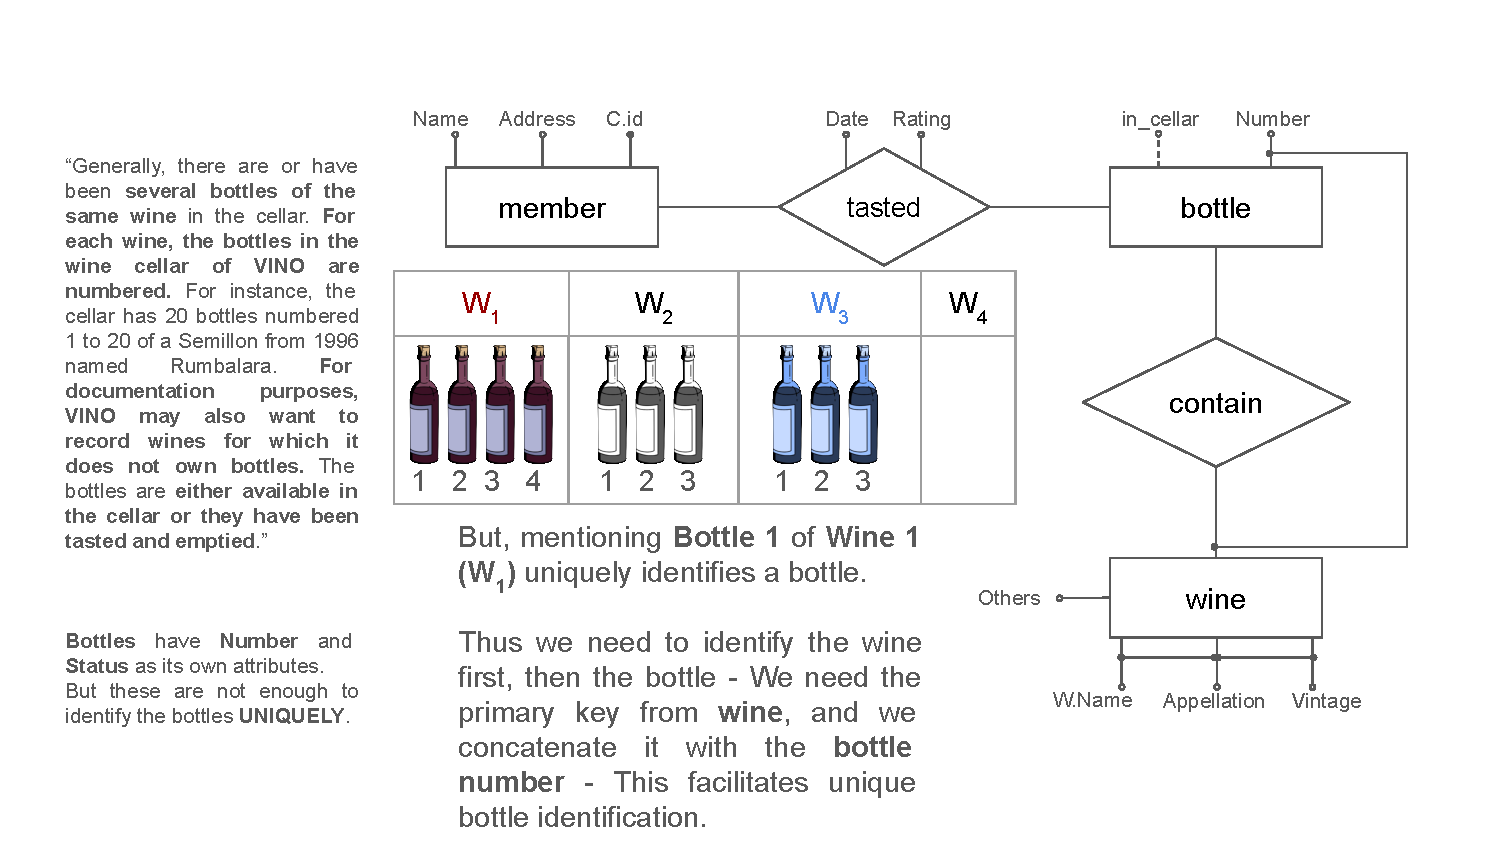
\includegraphics[width=1.1\linewidth]{tut_02_files/08.pdf}
    \end{figure}
\end{frame}

\begin{frame}
    \begin{figure}
        \centering
        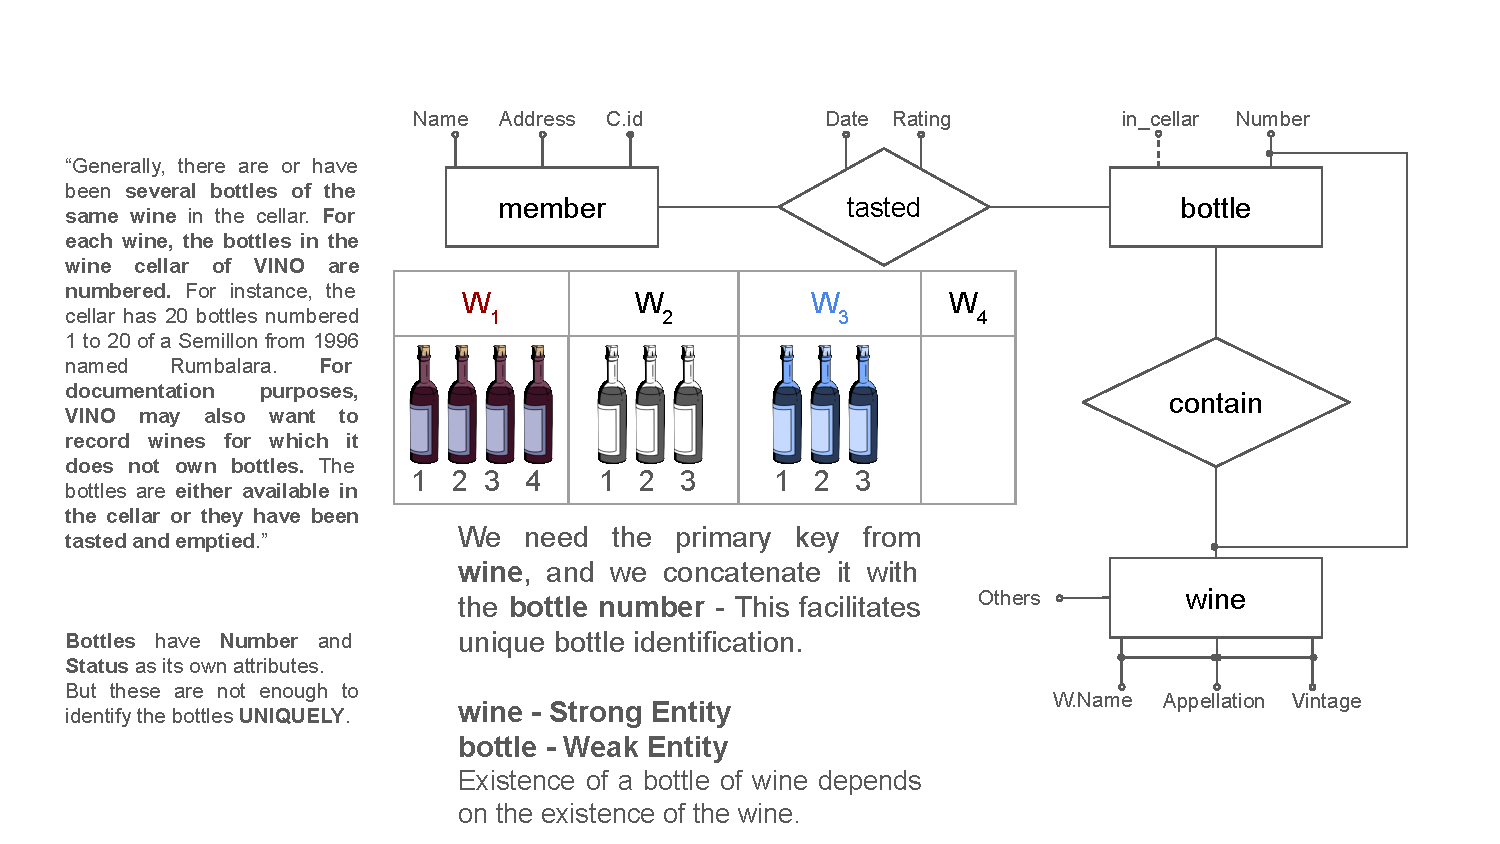
\includegraphics[width=1.1\linewidth]{tut_02_files/09.pdf}
    \end{figure}
\end{frame}

\begin{frame}
    \begin{figure}
        \centering
        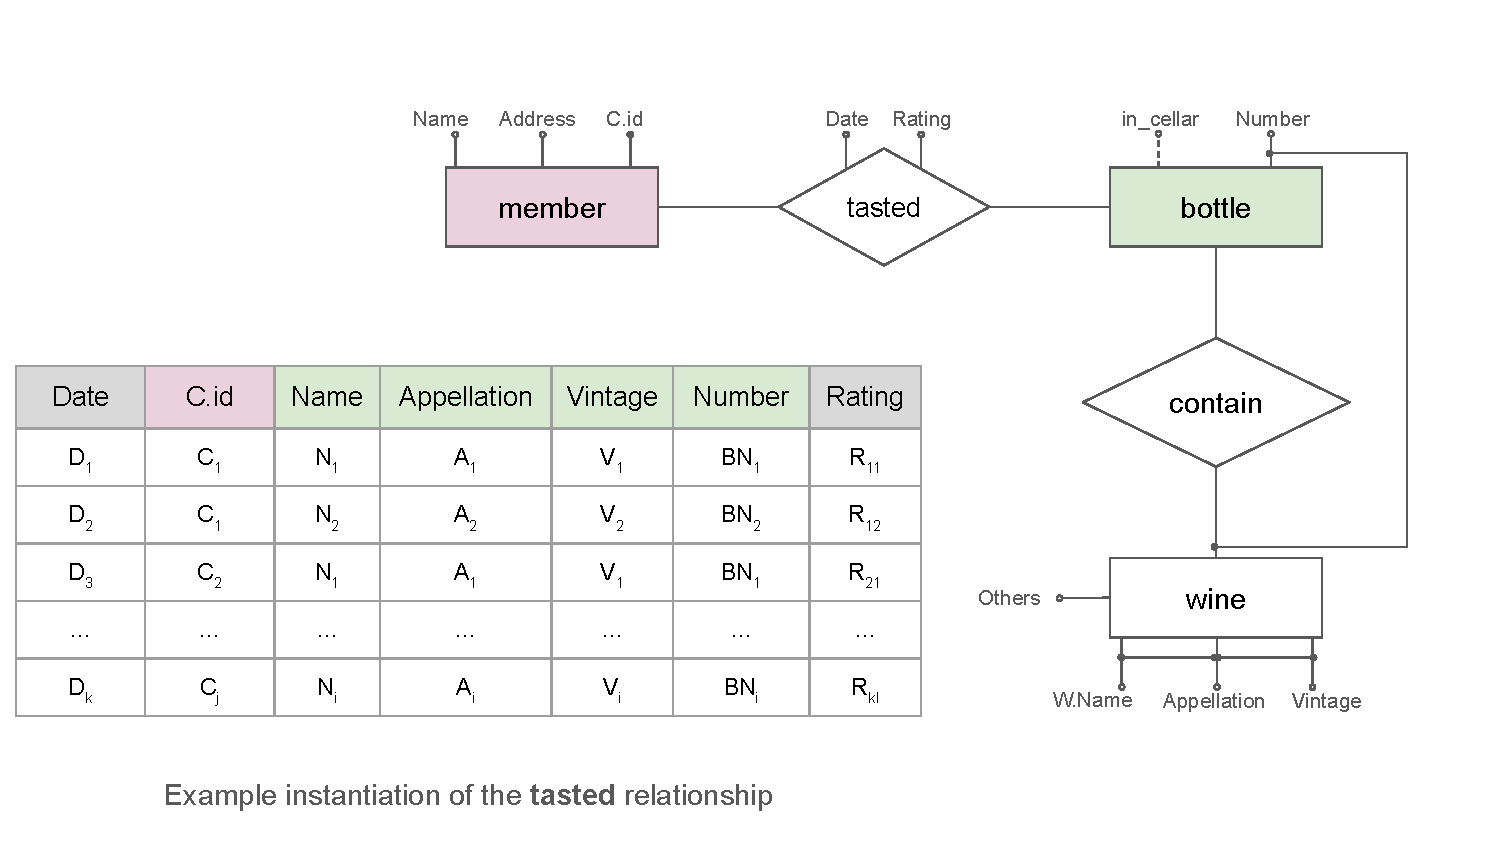
\includegraphics[width=1.1\linewidth]{tut_02_files/10.pdf}
    \end{figure}
\end{frame}

\begin{frame}
    \begin{figure}
        \centering
        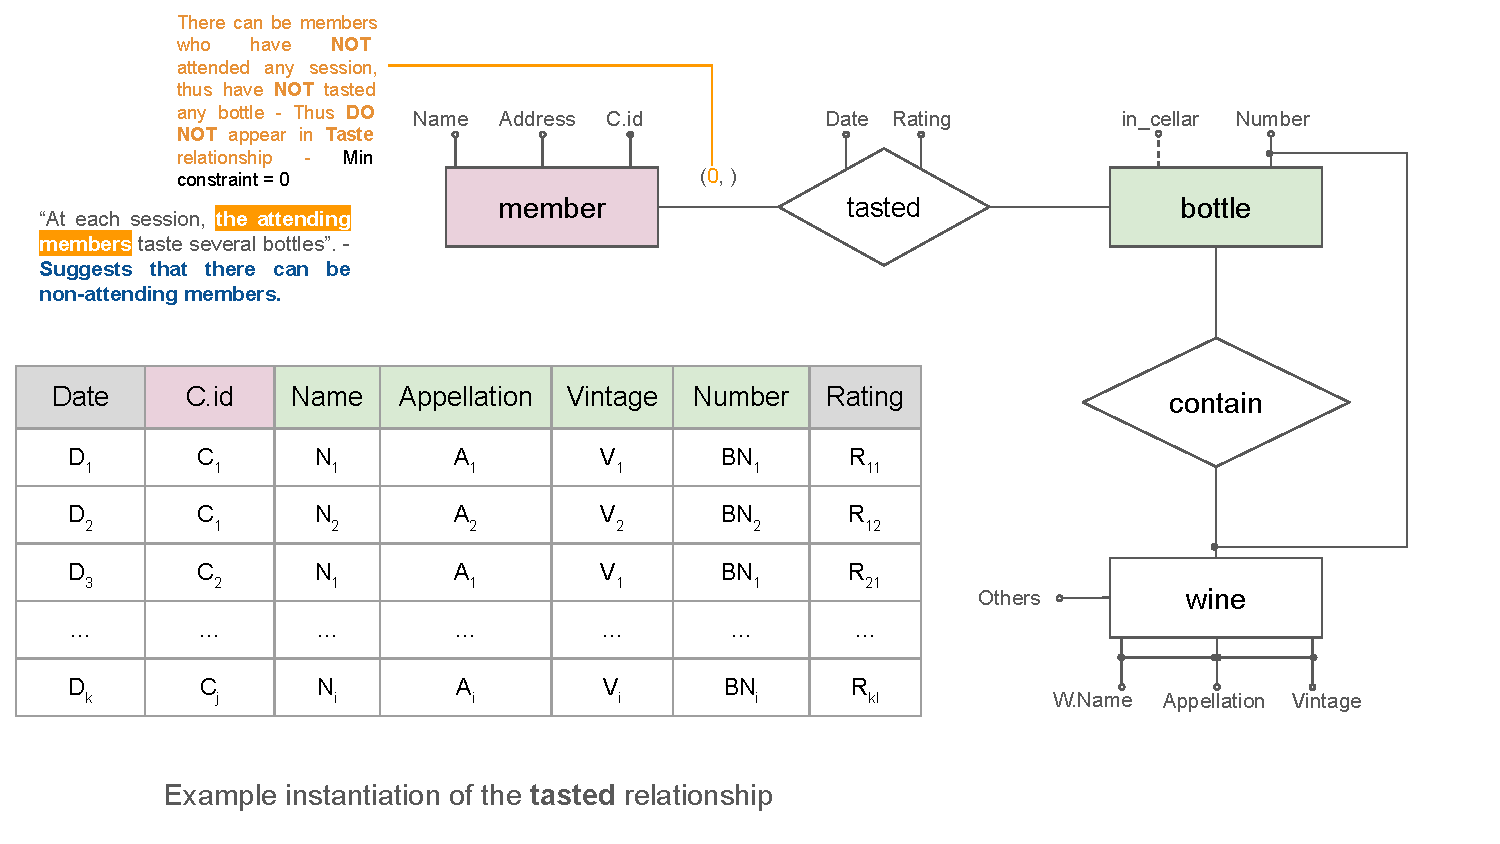
\includegraphics[width=1.1\linewidth]{tut_02_files/11.pdf}
    \end{figure}
\end{frame}

\begin{frame}
    \begin{figure}
        \centering
        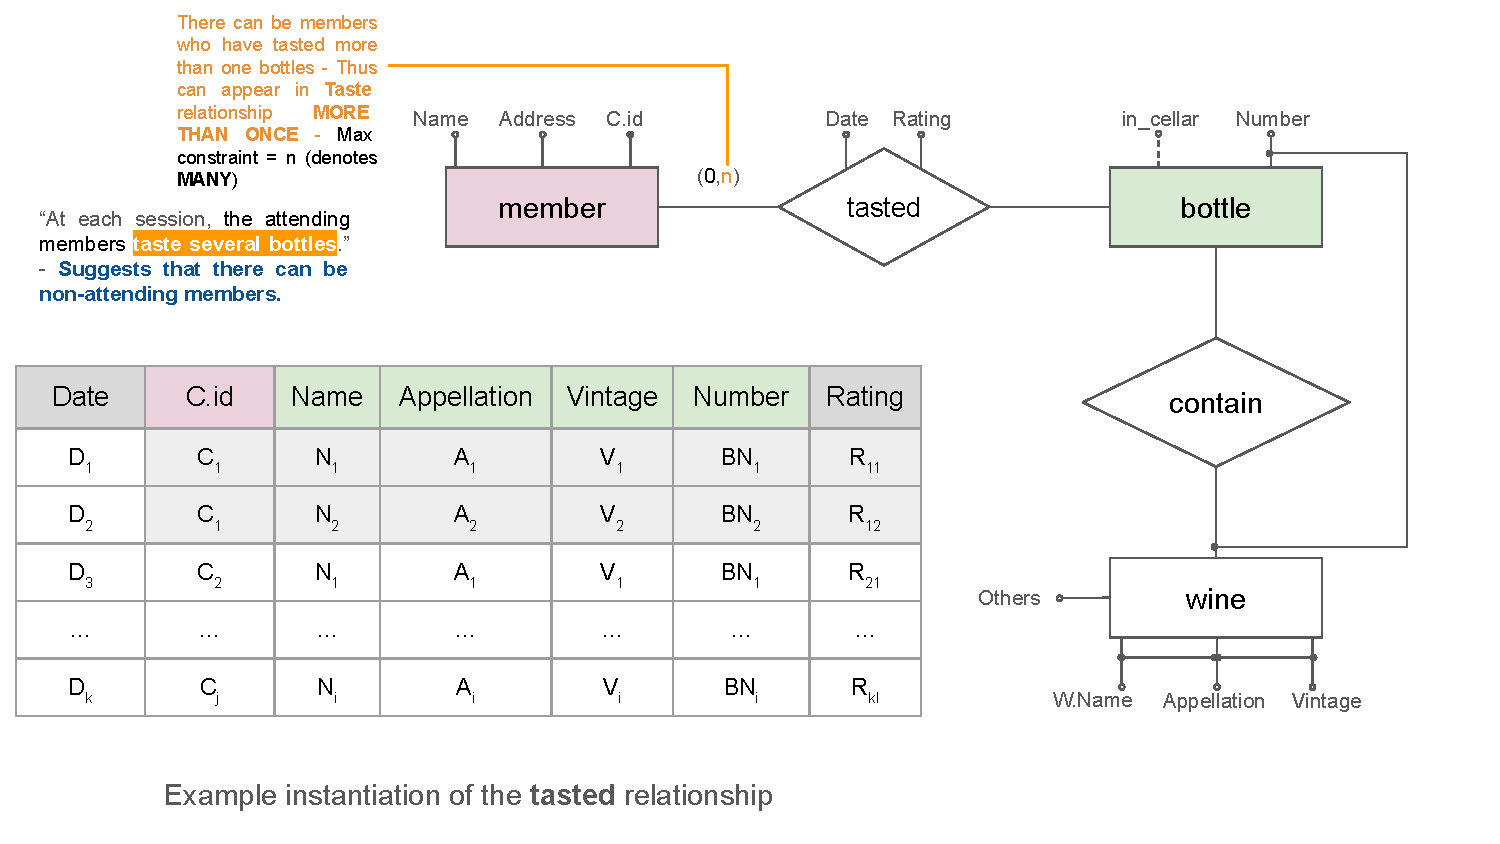
\includegraphics[width=1.1\linewidth]{tut_02_files/12.pdf}
    \end{figure}
\end{frame}

\begin{frame}
    \begin{figure}
        \centering
        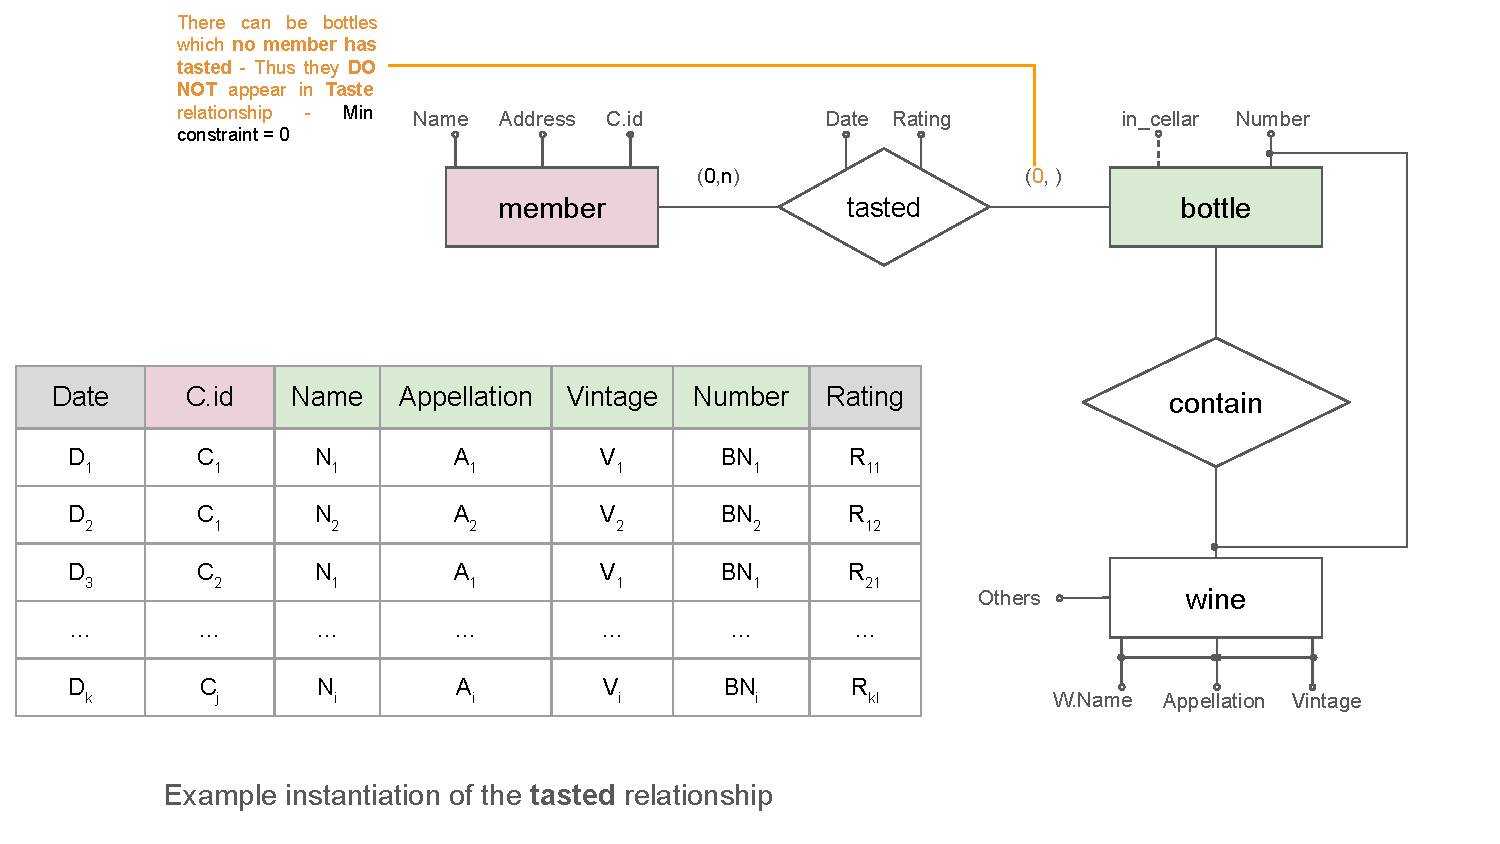
\includegraphics[width=1.1\linewidth]{tut_02_files/13.pdf}
    \end{figure}
\end{frame}

\begin{frame}
    \begin{figure}
        \centering
        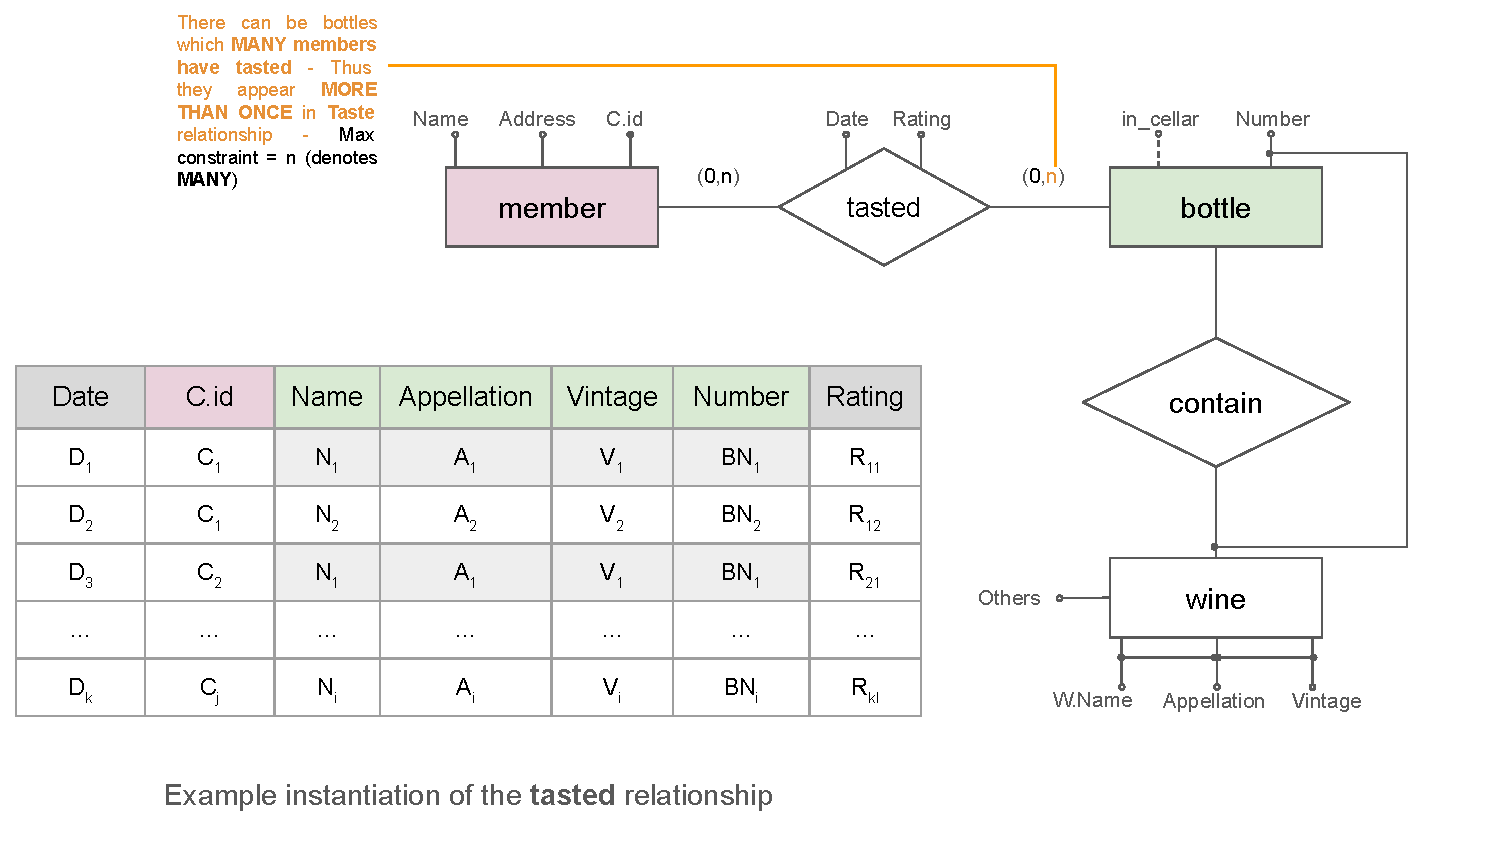
\includegraphics[width=1.1\linewidth]{tut_02_files/14.pdf}
    \end{figure}
\end{frame}

\begin{frame}
    \begin{figure}
        \centering
        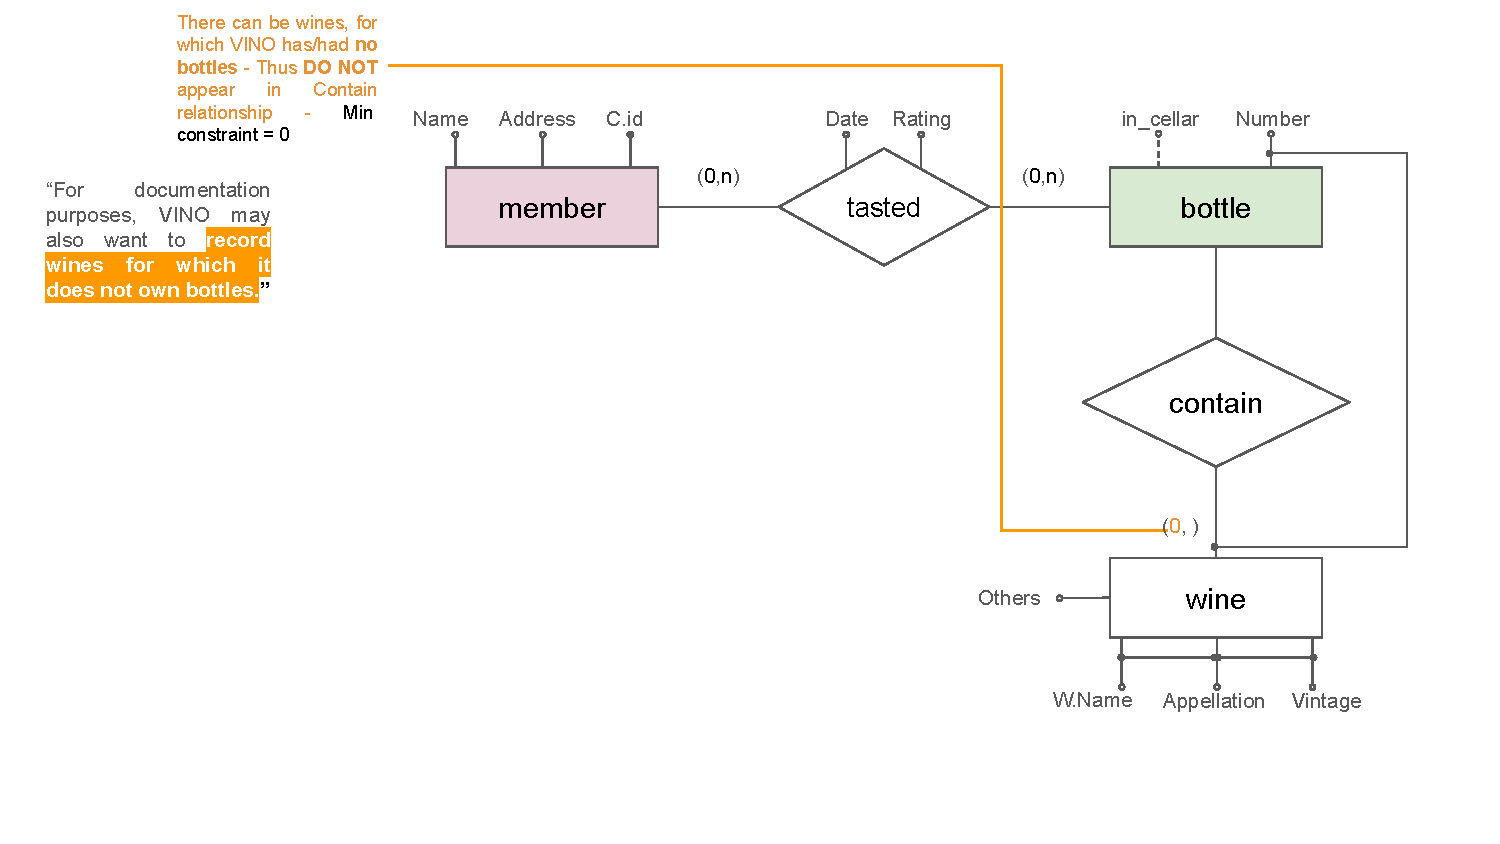
\includegraphics[width=1.1\linewidth]{tut_02_files/15.pdf}
    \end{figure}
\end{frame}

\begin{frame}
    \begin{figure}
        \centering
        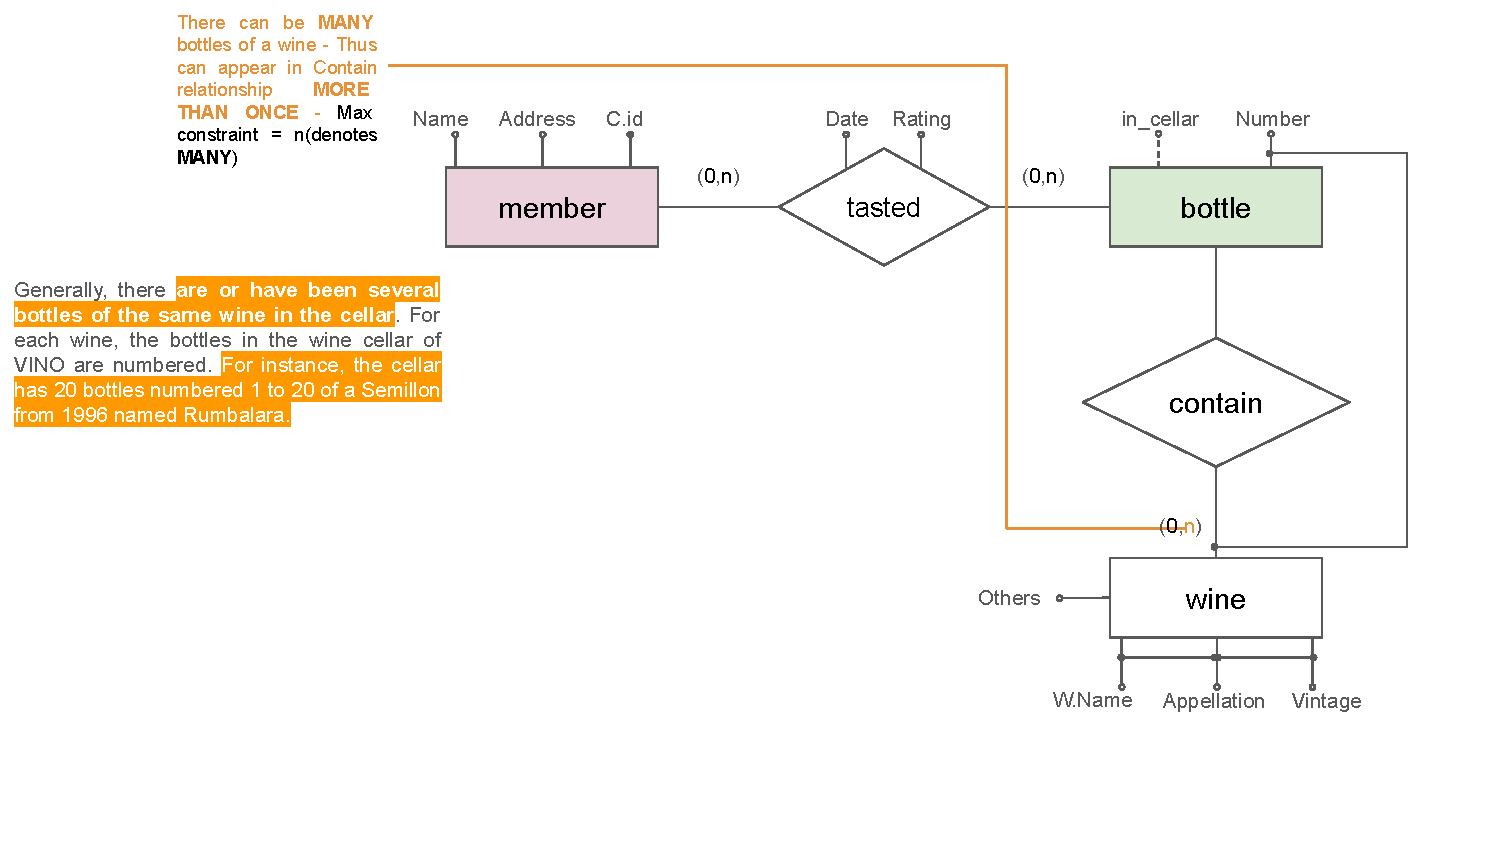
\includegraphics[width=1.1\linewidth]{tut_02_files/16.pdf}
    \end{figure}
\end{frame}

\begin{frame}
    \begin{figure}
        \centering
        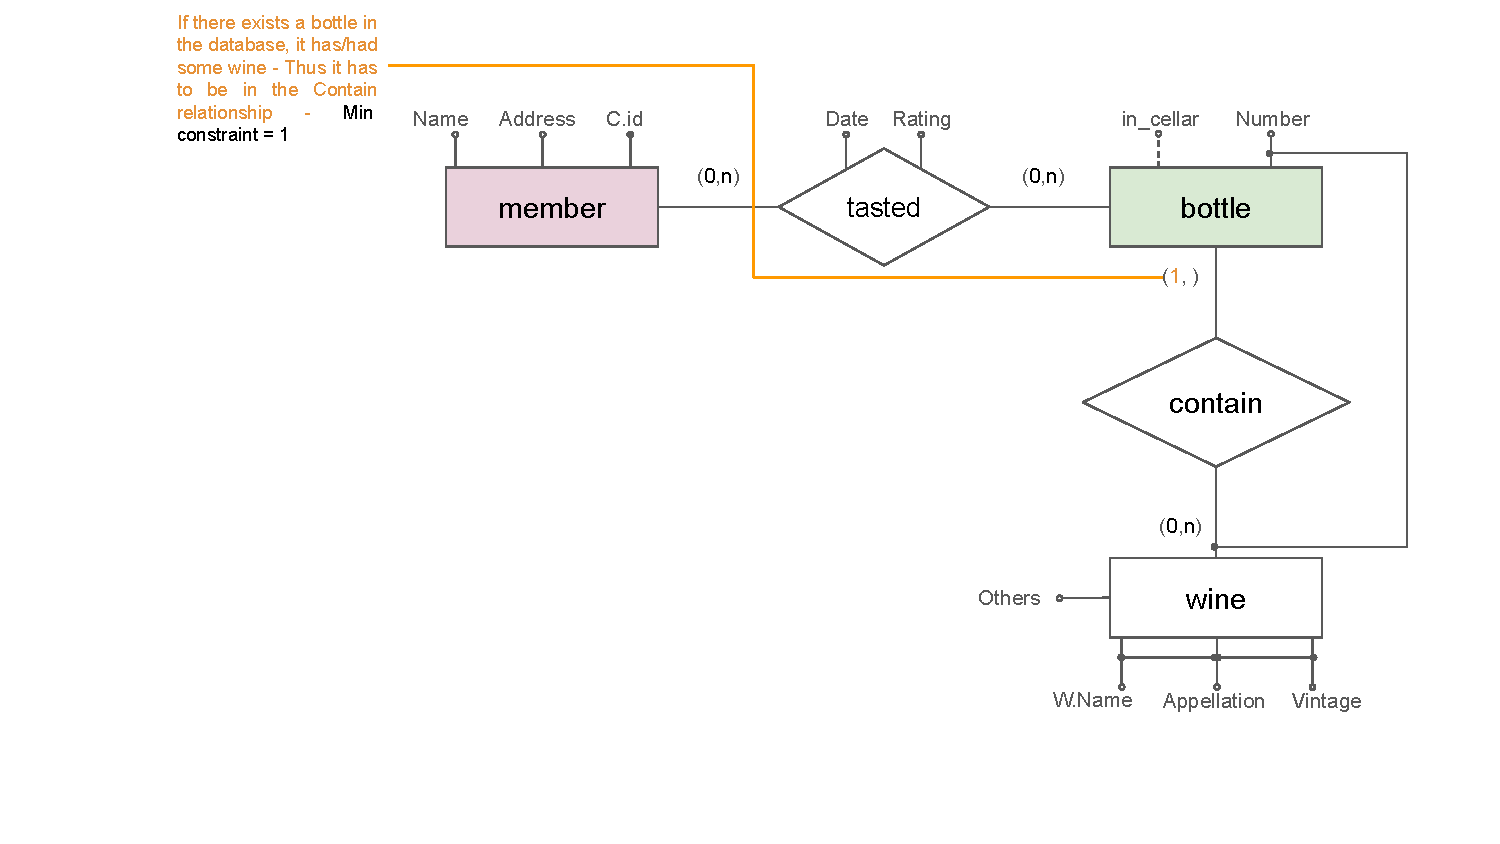
\includegraphics[width=1.1\linewidth]{tut_02_files/17.pdf}
    \end{figure}
\end{frame}

\begin{frame}
    \begin{figure}
        \centering
        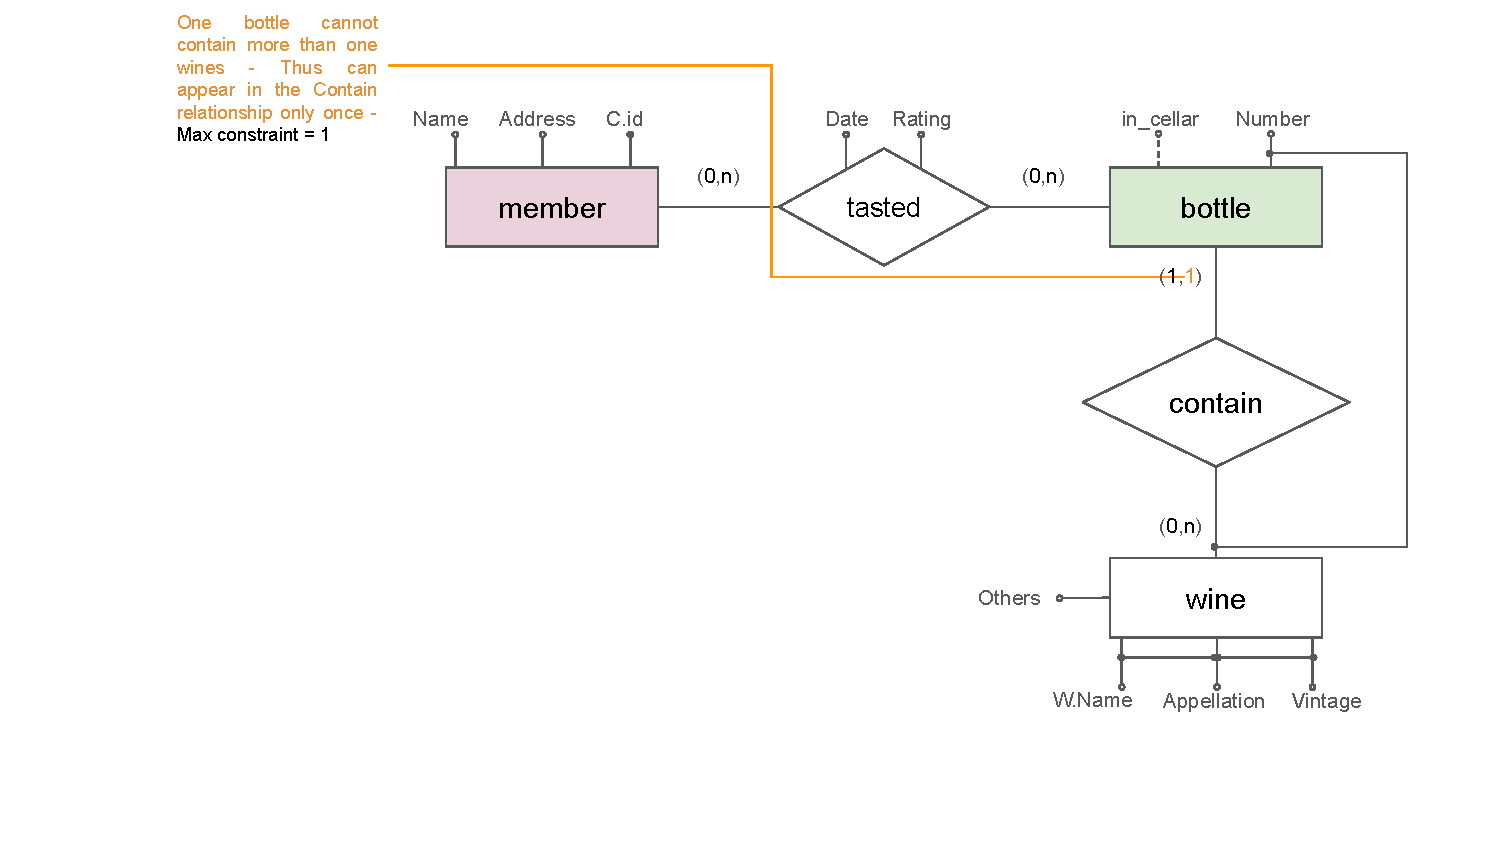
\includegraphics[width=1.1\linewidth]{tut_02_files/18.pdf}
    \end{figure}
\end{frame}

\begin{frame}
    \begin{figure}
        \centering
        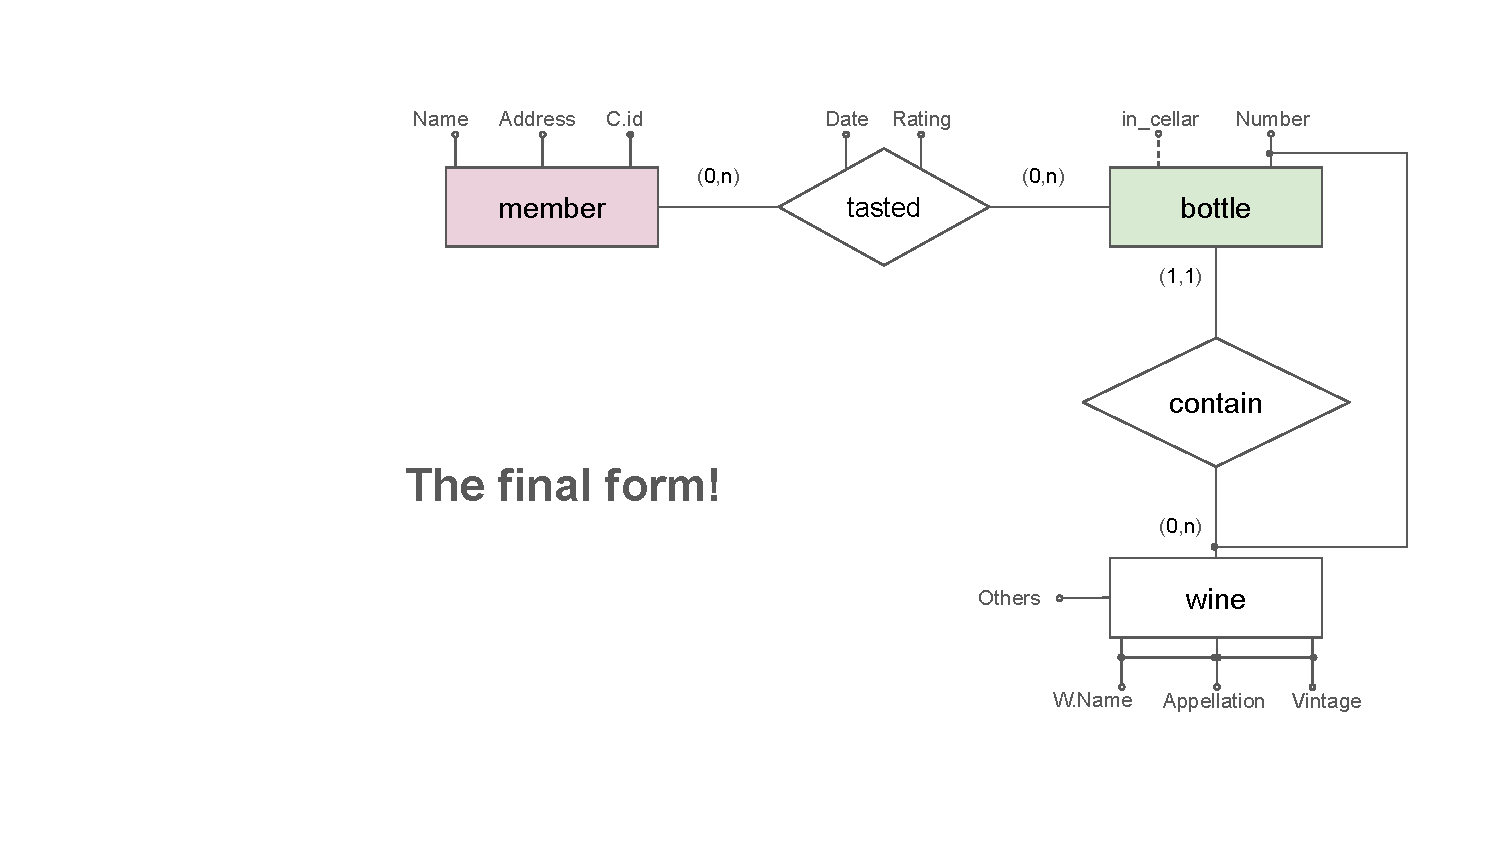
\includegraphics[width=1.1\linewidth]{tut_02_files/19.pdf}
    \end{figure}
\end{frame}

\begin{frame}
    \begin{figure}
        \centering
        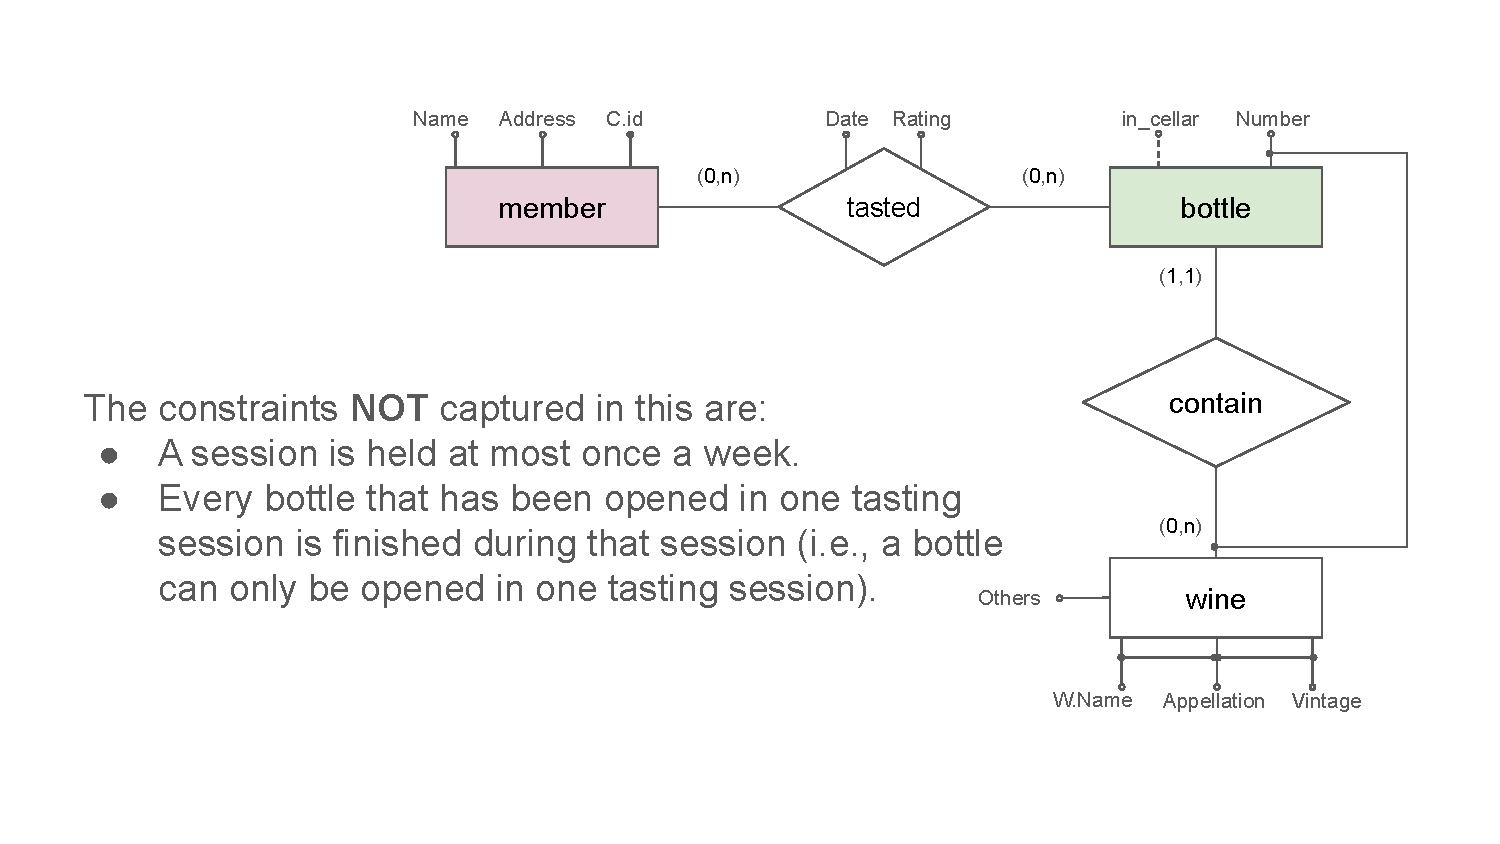
\includegraphics[width=1.1\linewidth]{tut_02_files/20.pdf}
    \end{figure}
\end{frame}

\begin{frame}
    \begin{figure}
        \centering
        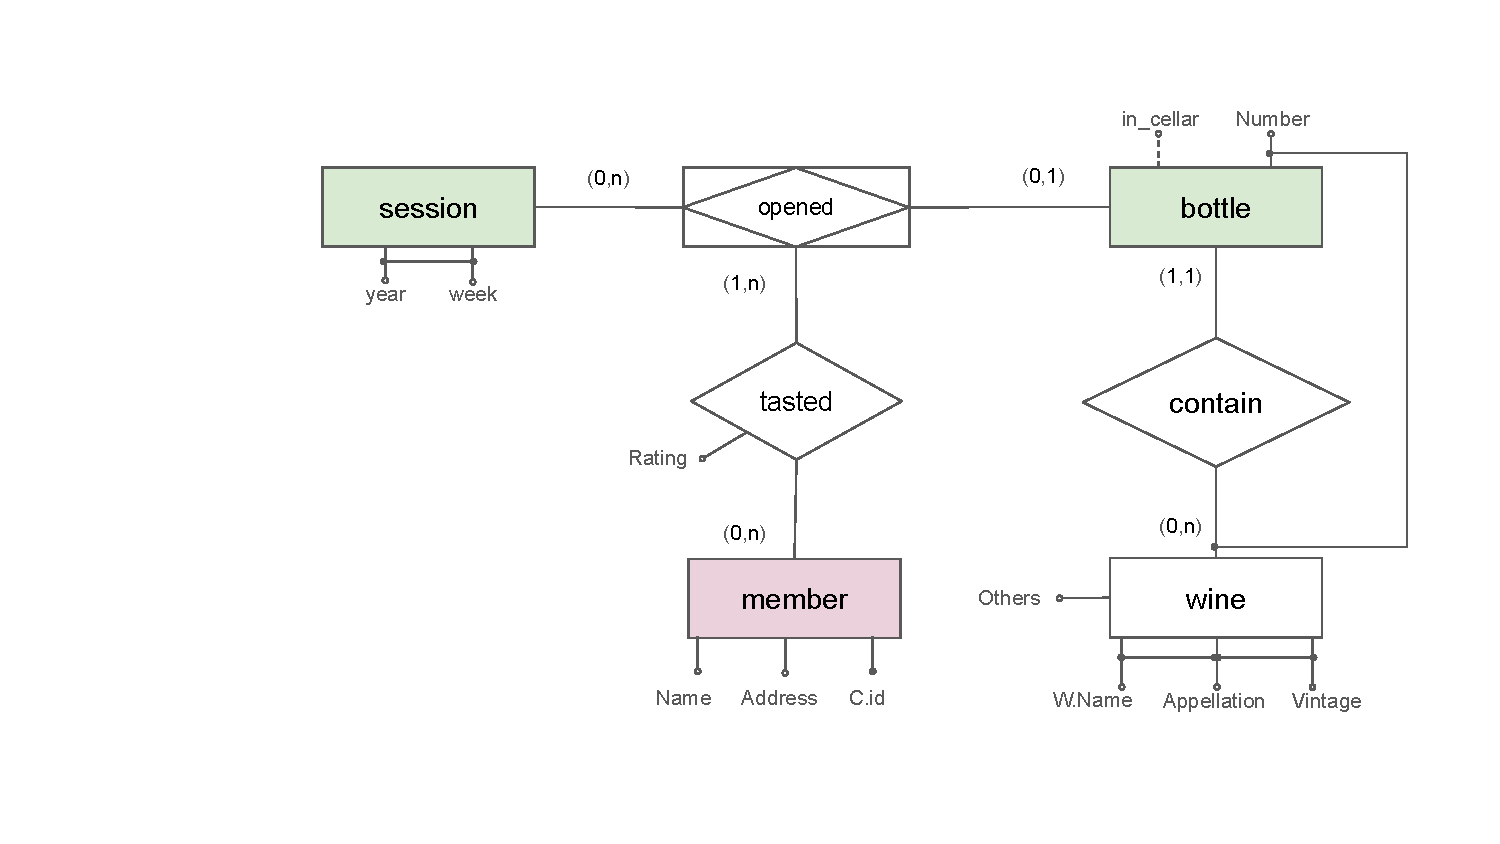
\includegraphics[width=1.1\linewidth]{tut_02_files/21.pdf}
    \end{figure}
\end{frame}
\end{document}